\documentclass[10pt, a4paper]{article}

\usepackage [T1]{fontenc}
\usepackage [utf8]{inputenc}
\usepackage [francais]{babel}

\usepackage {float}
\usepackage {graphicx}

\title {Cahier des besoins - Reversi}
\author {Guillaume CHUPIN, Benoit FAGET, Alexis PICHON, Julien PILLEUX}

\begin {document}
\maketitle
\thispagestyle {empty}
\newpage
\tableofcontents
\newpage

\section {Besoins fonctionnels}
\begin {itemize}
% Descriptions 'physiques' du programme.
\item L'utilisateur devra pouvoir jouer à une partie de Reversi dans une console de type bash lorsque il lance le programme.
\item La grille du jeu devra comporter des repères pour aider le joueur à choisir un mouvement à effectuer. Les cases en abscisses seront numérotées à l'aide de chiffres, et les cases en ordonnées seront numérotées à l'aide de lettres (voir FIGURE \ref{exemple_board}). Le joueur pourra alors choisir son mouvement en entrant dans la console la combinaison correspondante à la case souhaitée (ex : A2 ou a2).
\item Les cases vides de la grille devront être représentées grâce au caractère '\_', le joueur blanc sera représenté par un 'O' et le joueur noir par un 'X'. Les cases où le joueur courant peut effectuer son prochain coup, pourront être représentées par '*' (voir FIGURE \ref{exemple_board}). Ce plateau de jeu sera implémenté à l'aide d'une structure de donnée bitboard.
  % Image du plateau
  \begin {figure}[H]
    \centering
    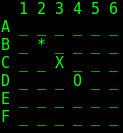
\includegraphics [scale = 0.5]{images/exemple_board.png}
    \label {exemple_board}
    \caption {Exemple de sauvegarde}
  \end   {figure}
  
  % Descritpion de l'option de sortie / sauvegarde.
\item A tout moment de la partie, le joueur peut décider de quitter le jeu et de sauvegarder l'état actuel du jeu en entrant 'Q' (ou 'q') dans la console. Lorsqu'il décide de faire ça, le programme donnera le choix à l'utilisateur de sauvegarder sa partie ou non. En entrant 'Y' (ou 'y'), le programme sauvegarde alors dans un fichier le tour du joueur courant ('X' ou 'O') ainsi que l'état du tableau actuel. Le fichier sera alors présenté de la même manière que le jeu mais sans la numérotation des cases ni l'aide pour le prochain coup du joueur (représenté par le caractère '*') (voir FIGURE \ref{exemple_save}). Le format de sorti de cette sauvegarde doit être sous format .txt. Si le joueur entre 'N' (ou 'n'), le programme ne sauvegarde donc pas le plateau. % Je n'ai pas marqué le format sur mes notes, confirmez svp :3
  % Image de la sauvegarde
  \begin {figure}[H]
    \centering
    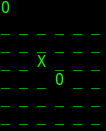
\includegraphics [scale = 0.5]{images/exemple_sauvegarde.png}
    \label {exemple_save}
    \caption {Exemple de sauvegarde}
  \end   {figure}
  
  % Options de lancement
\item Au lancement du programme, l'utilisateur doit pouvoir changer certains paramètres de la partie grâce à des options :
  \begin {description}
  \item [Taille du plateau de jeu] : Il sera possible de changer la taille du plateau de jeu avec l'option -s suivi d'un entier entre 1 et 4 (ex : -s3). Cette option fera donc varier la taille du plateau de 2 à 10 cases. Il sera donc impossible de rentrer des valeurs supérieures à 4 et inférieures à 1.
  \item [Le rôle de l'ordinateur]  : L'utilisateur pourra décider du rôle que l'ordinateur jouera pendant la partie, c'est à dire si il contrôle les blanc (-w), les noirs (-b), ou les deux (-a).
  \item [Un mode compétition]      : Il sera possible de démarrer le programme avec un mode compétition (-c). Cette option prend en entrée une sauvegarde d'un jeu, puis joue le prochain coup indiqué sur la sauvegarde.
  \end   {description}

  % IA
\item Le programme doit donc être capable de présenter une 'intelligence artificielle' pouvant affronter un joueur humain ou une autre machine. Celle-ci devra faire des choix de coup optimaux pour pouvoir vaincre son adversaire. Elle devra se baser sur un système de 'pondération de cases' lui permettant de faire un choix sur la quelle de ces cases avec la quelle elle a le plus de chances de gagner.
\end   {itemize}

\end   {document}
